%! Author = lili
%! Date = 6/4/26
\untit{Kapitel 15 in Lewin's Genes II}
% TODO unklar
% F 24 - 26, 60, 65 - 71

\section{Mobile genetische Elemente}\label{sec:mobile-genetische-elemente}

\subsection{Transposonen}\label{subsec:transposonen}
\defin{transposon}
% F 9 - 11 oder 13?

\begin{bsp}
    Transposonen beim Mais; Siehe Folie 12 -- 16
    % TODO F 15 - 16
\end{bsp}

\begin{figure}[H]
    \centering
    % \includegraphics[width=0.7\linewidth]{images/composite_transposon}
    \caption{Transposon}\label{fig:composite_transposon}
\end{figure}

\subsubsection{Kategorisierung}
\defin{transposon_klasse_i}
\defin{transposon_klasse_ii}

\gls{transposon_klasse_ii}s kommen in Pro- und Eukaryoten vor.
Eukaryotische Genome zeigen i.d.R. hohe Anzahl und Vielfalt an
Transposons, aber viele sind defekt und zeigen keine (unabhängige) Transposition
mehr.

Sie können autonom oder nicht-autonom sein.

\begin{figure}[H]
    \centering
    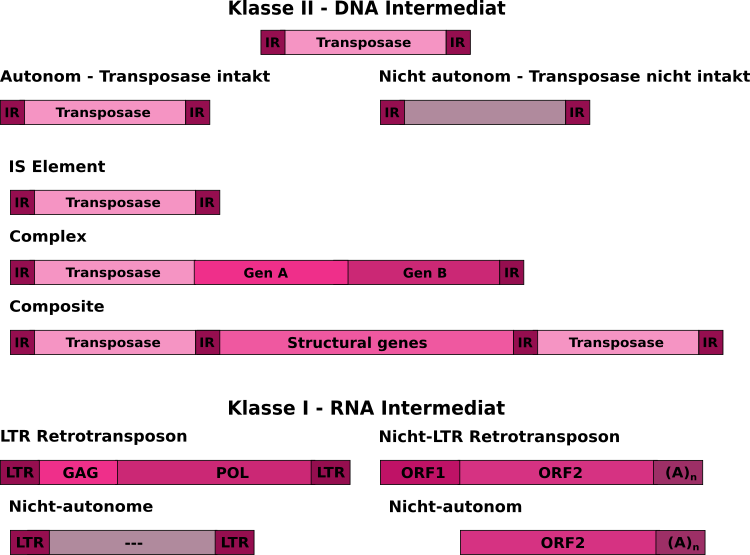
\includegraphics[width=0.9\linewidth]{images/transposon_klassen}
    \caption{Kategorisierung auf Aufbau von Transposons}\label{fig:transposon_klassen}
\end{figure}



% TODO Karteikarte unterchied der verbreitung der klasse I und II

% TODO F 17 - 18
\begin{bsp}
    Wichtige Transposon-Familien aus Mais
        % TODO F 19 - 20
\end{bsp}

\kfrage{autonomietransposon}

\subsubsection{Transpositionsmechanismus}
% TODO F 22 - 23

\begin{bsp}
    Anwendung: Transposon tagging
        % TODO F 21, 27
\end{bsp}

\subsubsection{Aktivität von Transposons}
% TODO F 28, 42 - 46

\subsection{Retrotransposons und Retroviren}\label{subsec:retrotransposons-und-retroviren}
% TODO F 30

\subsubsection{Aufbau}
% TODO F 32 - 33

\subsubsection{Stadien}
% TODO F 34 - 37

\subsubsection{Retroviraler Lebenszyklus}
% TODO F 31

\subsubsection{Typen}
% TODO F 38

\subsubsection{Funktion}
% TODO F 39

\begin{bsp}
    Repetitive DNA im Humangenom / TE-Gehalt von 248 Säugetier GSeq-Assemblies
        % TODO F 40 - 41
\end{bsp}

\section{Methoden der DNA-Übertragung}\label{sec:methoden-der-dna-ubertragung}
% TODO F 48

\begin{bsp}
    A plant tumor of bacterial origin
    % TODO F 49 - 51 
\end{bsp}

\subsection{T-DNA Transformation}\label{subsec:t-dna-transformation}
% TODO F 52 - 53
\subsubsection{Ti-Plasmide}
% TODO F 54 - 55

\subsubsection{Ablauf}
% TODO F 56 - 57, 61

\subsubsection{Struktur und Funktion der T-DNA Enden}
% TODO F 58 - 59

\subsubsection{Binäre Vektorsysteme}
% TODO F 62

\subsubsection{Transformation von Arabidopsis}
% TODO F 63 - 64


%%
\kfrage{aktivtransposon}
